%
% File emnlp2015.tex
%
% Contact: daniele.pighin@gmail.com
%%
%% Based on the style files for ACL-2015, which were, in turn,
%% Based on the style files for ACL-2014, which were, in turn,
%% Based on the style files for ACL-2013, which were, in turn,
%% Based on the style files for ACL-2012, which were, in turn,
%% based on the style files for ACL-2011, which were, in turn, 
%% based on the style files for ACL-2010, which were, in turn, 
%% based on the style files for ACL-IJCNLP-2009, which were, in turn,
%% based on the style files for EACL-2009 and IJCNLP-2008...

%% Based on the style files for EACL 2006 by 
%%e.agirre@ehu.es or Sergi.Balari@uab.es
%% and that of ACL 08 by Joakim Nivre and Noah Smith

\documentclass[11pt,a4paper]{article}
\widowpenalty=10000
\clubpenalty=10000
\usepackage{acl2015}
\usepackage{times}
\usepackage{url}
\usepackage{latexsym}
\usepackage{color}
\usepackage{enumitem}
\usepackage{booktabs}
\usepackage{graphicx}
\usepackage{todonotes}
\usepackage[utf8]{inputenc}


%\setlength\titlebox{5cm}

% You can expand the titlebox if you need extra space
% to show all the authors. Please do not make the titlebox
% smaller than 5cm (the original size); we will check this
% in the camera-ready version and ask you to change it back.


\title{Predicting word sense annotation agreement}

%\author{Héctor Martínez Alonso$\ddagger$ Anders Johannsen \\
%  Affiliation / Address line 1 \\
%  Affiliation / Address line 2 \\
%  Affiliation / Address line 3 \\
%  {\tt email@domain} \\\And
%  Oier Lopez de Lacalle  Eneko Agirre$\dagger$ \\
%  Affiliation / Address line 1 \\
%  Affiliation / Address line 2 \\
%  Affiliation / Address line 3 \\
%  {\tt email@domain} \\}
  
  \author{Héctor Martínez Alonso$\dagger$ \quad Anders Johannsen$\dagger$ \quad Oier Lopez de Lacalle$\ddagger$ \quad Eneko Agirre$\ddagger$ \\
%\quad University of Copenhagen \quad \quad \quad \quad  \quad \quad \quad \quad \quad \quad \quad  University of the Basque Country \\
 $\dagger$University of Copenhagen \\ $\ddagger$University of the Basque Country \\
  {  {\normalsize \{{\tt alonso,johannsen\}@hum.ku.dk \{{\tt e.agirre,oier.lopezdelacalle\}@ehu.eus}}}} }
   

\date{}

\begin{document}
\maketitle
\begin{abstract}


High agreement is a common objective when annotating data for word senses.  
However, a number of factors make perfect agreement impossible, e.g.\ the limitations of sense inventories, the difficulty of the examples or the interpretation pre\-ferences of the annotators.
Estimating potential agreement is thus a relevant task to supplement the evaluation of sense annotations.
In this article we propose two methods to predict agreement on word-annotation instances. We experiment with a continuous representation and a three-way discretization of observed agreement. In spite of the difficulty of the task, we find that different levels of agreement can be identified---in particular, low-agreement examples are easier to identify.
\end{abstract}
\section{Introduction}

Sense-annotation tasks show less-than-perfect agreement scores. However, variation in agreement is not the result of featureless, white noise in the annotations; \newcite{krippendorff2011} defines disagreement as \textit{by chance}---caused by unavoidable inconsistencies in annotator behavior---and \textit{systematic}---caused by properties of the data.

Our goal is to predict the agreement of sense-annotated examples by examining their linguistic properties. If we can identify properties predictive of low or high agreement, then we can claim that some of the agreement variation in the data is indeed systematic. %, and is a result of the interplay between the linguistic properties of the examples and the characteristics of the sense inventory.



\newcite{Artstein2008} provide an interpretation of Kripperdorff's $\alpha$ coefficient to describe the reliability of a whole annotation task and the way that observed agreement ($A_o$) is calculated for each example. Strictly speaking, the value of $\alpha$ only provides an indication of the replicability of an annotation task, but we propose that the difficulty of annotating a particular example will influence its local observed agreement. Thus, easy examples will have a high $A_o$, that will be lower for more difficult examples. 


%The goal of this experiment is to measure how much of the disagreement in the annotations is caused by linguistic properties of the examples and is thus systematic. More specifically, we intend to interpret the $R^2$ determination coefficient of a regression model on the linguistic features.1



Identifying low-agreement examples by their linguistic features would help characterize contexts that make words difficult to annotate. Estimating the agreement of examples has an immediate application for data collection, as a way of estimating the proportion of examples of each difficulty level that one wants to sample. Moreover, a model of (dis)agreement can help interpret the mispredictions of a word-sense disambiguation system without requiring the data to be multiply annotated. 

Observed agreement $A_o$ is a continuous-valued variable in the unit interval and we tackle its prediction as a regression task (Section \ref{sec:reg}). We also experiment with a discretized version of observed agreement into low, mid and high agreement, which is predicted using classification (Section \ref{sec:class}).  

\section{Related work}

In their study, \newcite{Yarowsky2002} examine the relation between agreement variation and predictive power of word-sense disambiguation systems, which is later expanded by \newcite{Lopez2015}. Our work is different in that we do not study the relation between agreement and performance, but between example properties and agreement. \newcite{alonso2013annotation} experiments with prediction of agreement for coarse-sense annotation. 

\newcite{Tomuro2001} uses the disagreement between annotators of two English sense-annotated corpora to provide insights on the relations between synsets, and more recent studies \cite{Jurgens2013,Plank2014,Jurgens2014,lopezdelacalleagirre2015} have empirically tackled the issue of inter-annotator disagreement as a phenomenon that is potentially informative for natural language processing. Other research efforts advocate for models of annotator behavior \cite{passonneau2009making,Passenau2010,Passonneau2014,Cohn2013}. 

\section{Data}
%\subsection{Datasets}
We conduct our study on sense-annotated datasets, keeping only the examples with at least two annotations per item. 
%Sometimes a whole dataset is multiply annotated. 
%In the datasets with two annotators and one adjudicator, we disregard adjudications because they potentially have a bias that is different from the the annotators'.
In the datasets with two annotators and one adjudicator, we disregard adjudications given their potentially different bias.

\begin{itemize}[nolistsep,noitemsep]
\item[\textbf{1}] \textsc{mascc} The English crowdsourced lexical-sample word-sense corpus from \newcite{Passonneau2014}.
\item[\textbf{2-5}] \textsc{masce*} The expert annotations for a series of English lexical-sample words from \newcite{Passonneau2012}, with several annotation rounds. We include the second, third and fourth round of annotation in our experiments. We use on the whole dataset (\textsc{Mascew}) pooling all the rounds together, as well as on each round independently, namely \textsc{masce2}, \textsc{masce3} and \textsc{Masce4}.
\item[\textbf{6}] \textsc{Fntw} The English Twitter FrameNet data of \newcite{Sogaard2015}. We treat the frame-name layer as a word-sense layer, and disregard the arguments.
\item[\textbf{7}] \textsc{Ensst} The English supersense-annotated data of \newcite{Johannsen2014}.
\item[\textbf{8}] \textsc{Eusc} The Basque lexical-sample SemCor of \newcite{Agirre2006}.
\item[\textbf{9}] \textsc{Dasst} The Danish supersense-annotated  data of \newcite{MartinezAlonso2015}.
\end{itemize}
Table \ref{tab:data} provides the characteristics of the datasets. The annotation task can be lexical-sample (ls) or all-words (aw). The number of instances is different from the number of sentences for all-words annotation. The type of annotators can be expert (ex) or crowdsourced (cs). The $\alpha$ scores can differ from those reported in the datasets' documentation given our example-selection criteria. The last two columns describe the target variables of observed agreement ($A_o$) and the proportion of low-, mid- and high-agreement instances, cf. \ref{sec:targetvariable} for details.

\begin{table*}[Ht!]

\begin{center}
  \begin{tabular}{llllrrrcccc}
  \toprule 

Dataset& lang & inventory & task & sent & inst & ann & type & $\alpha$ & $A_o\pm\sigma$ & \textsc{l/m/h}\\ 
\midrule 

\textsc{mascc} & English & synset & ls & 44.6k & 44.6k & 13-25 & cs & .40 & .14 $\pm$ .24 & 25/44/31\\
\textsc{mascew} & English & synset & ls & 2.6k & 2.6k & 2-6 & ex & .48 & .07 $\pm$ .35 & 24/21/55\\
---\textsc{masce2} & English & synset & ls & 1.5k & 1.5k & 5-6 & ex & .51 & .41 $\pm$ .30 & 21/36/43\\
---\textsc{masce3} & English & synset & ls & 500 & 500 & 3 & ex & .69 & .80 $\pm$ .33 & 28/\textcolor{gray}{00}/72\\
---\textsc{macse4} & English & synset & ls & 618 & 618 & 2 & ex & .63 & .73 $\pm$ .44 & 27/\textcolor{gray}{00}/73\\
\textsc{ensst} & English & supersense & aw & 39 & 326 & 3 & ex & .67 & .69 $\pm$ .36 & 45/\textcolor{gray}{00}/55\\
\textsc{fntw} & English & frame & aw & 236 & 958 & 3 & ex & .82 & .82 $\pm$ .31 & 26/\textcolor{gray}{00}/74\\

\textsc{eusc} & Basque & synset & ls & 20.6k & 20.6k & 2 & ex & .76 & .76 $\pm$ .43 & 24/\textcolor{gray}{00}/76\\
\textsc{dasst} & Danish & supersense & aw & 1.2k & 9.5k & 2 & ex & .65 & .67 $\pm$ .47 & 33/\textcolor{gray}{00}/67\\


\bottomrule

  \end{tabular}  
\end{center}
\caption{Dataset characteristics \label{tab:data} in terms of language, sense inventory, task (al:all-words, ls:lexical sample), no. of sentences, no. of instances, no. of annotators, type of annotators (ex:expert,cs:crowdsourced), $\alpha$, observed agreement and percentage of \textsc{low/mid/high} agreement examples.}
\end{table*} 

\subsection{Features}
We define an \textit{instance} as a sentence with a target word for annotation. If a sentence has $n$ annotated target words, it yields $n$ instances. For each instance, we obtain features for a word $w$ and its syntactic parent $p$ in a sentence $s$, organized in feature groups. The word identities of $w$ and $p$ are not included in the features to keep the models more general. Number of features are in parentheses.\\ 
\noindent\textbf{Frequency(2)} We calculate the frequency of $w$ and $p$, scaling by $log(rank(x)+1)^{-1}$.\\
\textbf{ Morphology (5)} We consider the part-of-speech tag (POS) of $w$, of $p$, and the POS-bigram at the left and at the right of $w$. In order to incorporate information on inflectional complexity, we calculate which proportion of the frequency of the stem of $w$ is covered by $w$, e.g.\ the occurrences of `jumping' constitute 22\% of the occurrences of the stem `jump'. \\
\textbf{Syntax (5)} We calculate the number of dependents of $w$ and $p$, and a bag of words for the labels of the dependents of $w$ and $p$. We also include the distance from $w$ to the root node, and the linear distance between $w$ and $p$.\\
\textbf{ Context  (5)} We calculate the length of $s$ in tokens, the proportion of $w$ made up of content words, and a bag of words of the context of $w$, i.e.\ all the words of $s$ except $w$. To capture context specificity, we calculate the maximum and the sum of the sentence-wise idf of each stem in $s$. \\
\textbf{Sense inventory (2)} We calculate the number of possible senses for $w$, plus an additional sense when $w$ could be discarded from the annotation---like the tag `O' for supersenses---or the right synset was not present in WordNet. We also calculate the sense entropy for each word following \newcite{Yarowsky2002}. 

 We use TreeTagger \cite{Schmid1994} for POS tagging and TurboParser \cite{Martins2010} for dependency parsing, both trained on Universal Dependencies v1.1,\footnote{\url{https://lindat.mff.cuni.cz/repository/xmlui/handle/11234/LRT-1478}} to allow cross-language feature comparison. %We estimate frequencies on 100M-word web-crawled and Wikipedia corpora for English and Danish, and on 13M newswire for Basque. We perform Snowball stemming. 
 We estimate frequencies on a 100M-word corpus for English \cite{ferraresi2008introducing} and Danish \cite{Asmussen2012}, and on 13M for Basque \cite{leturia:2012}, using Snowball stemming.

\subsection{Target variable}
\label{sec:targetvariable}
\paragraph*{Regression} Instance-wise observed agreement ($A_o$) is the target variable for the regression experiments. We obtain  $A_o$ for each example by counting the pairwise matches in the annotation and dividing over the amount of pairwise combinations. 
Note that  $\alpha$ is an aggregate measure that is obtained dataset-wise, and $A_o$ is the only agreement measure available for individual instances.
%\paragraph*{Classification} Agreement level is the target variable for the classification experiments, where we discretize $A_o$ into the three classes, namely LOW, MID and HIGH. We set the threshold for LOW at $Ao \le \frac{1}{3}$, for HIGH at $Ao \ge \frac{2}{3}$, and intermediate values receive the label MID. Instances with MID value first appear for more than three annotators (cf. Table \ref{tab:data}.

\paragraph*{Classification} The target variable for the classification experiments is a discretization of $A_o$ into three agreement-level classes, namely \textsc{low}, \textsc{mid} and \textsc{high}. The threshold for \textsc{low} is set at $A_o \le \frac{1}{3}$, and for \textsc{high} at $A_o \ge \frac{2}{3}$. The \textsc{mid} value is only possible for datasets with more than three annotators (cf. Table \ref{tab:data}).



\section{Experiments}
We use the scikit-learn\footnote{\url{http://scikit-learn.org/}} implementation for all learning algorithms, and train and test on 10-fold cross validation.
\paragraph{Regression} We use L2-regularized linear regression. 
%The output of the regression is sigmoid-transformed to keep the values in the range $[0,1]$. 
The baselines for regression are \textsc{mean}, where all instances receive the mean $A_o$ of the dataset, and  \textsc{median}, that assigns the median $A_o$. 
\paragraph{Classification} We use a maximum-entropy classifier. The baselines for classification are \textsc{mfc}, where all instances receive most frequent class, and the two random baselines: \textsc{stra}, where the assigned values are randomly selected via stratified sampling from the distribution of classes in the dataset, and \textsc{uni} where values are assigned from the uniform distribution of the three labels. 

\subsection{Regression}
\label{sec:reg}
Table \ref{tab:regagr_results} shows the results for regression in terms of mean absolute error (MAE). This metric is more suitable than root-mean-square error (RMSE) when evaluating regression in the [0,1] interval. Datasets where the system outperforms both baselines are in bold.


\begin{table}[Ht!]

\begin{center}
  \begin{tabular}{lc|cc}
 \toprule
 & \textsc{Regression} & \textsc{mean} & \textsc{median} \\
 \midrule
 \textsc{mascc} & \textbf{0.19} & 0.21 & 0.21 \\
 \textsc{mascew} & \textbf{0.31} & 0.32 & 0.37 \\
---\textsc{masce2} & {0.27} & 0.26 & 0.25 \\
---\textsc{masce3} & {0.36} & 0.29 & 0.20 \\
---\textsc{masce4} & {0.46} & 0.40 & 0.27 \\
\textsc{ensst} & {0.43} & 0.35 & 0.31 \\
\textsc{fntw} & {0.27} & 0.26 & 0.18 \\

\textsc{eusc} & 0.35 & 0.37 & 0.24 \\
\textsc{dasst} & 0.42 & 0.44 & 0.33 \\

\bottomrule

  \end{tabular}  
\end{center}
\caption{Mean absolute error of prediction for regression and for mean and median baselines. Datasets where the system outperforms the best-performing baseline are marked in bold. \label{tab:regagr_results}}
\end{table} 

The results for regression show that predicting instance-wise $A_o$ is a hard task. The learnability of the task is limited by the resolution of the target variable; the only two datasets that can beat all baselines (and thus have lower MAE) have many instances, and many annotators (about 50\% of the instances in \textsc{mascew} have five or more annotators). Also, size of the dataset is a relevant factor for a good estimation of $A_o$.

We also examine goodness of fit in terms of $R^2$ (determination coefficient or explained variance). $R^2$ does not strictly say how much agreement is systematic, but how much of the agreement variation within a dataset can be explained by the features. The only two datasets with positive $R^2$ are \textsc{mascc} and \textsc{eusc}, at .082 and 0.014 respectively. \textsc{eusc} has only two annotators per instance, but it is a large dataset that allows mapping some properties of the features onto the variance of $A_o$.

The two datasets with a goodness of fit over baseline are the largest ones. This behavior indicates that the regression method suffers from the data bottleneck. Smooth estimation of continuous values might be more sensitive to data volume than estimation of discrete values, therefore we experiment with classification in the next section.

%We will consider the proportion of explained variance of the regression model described by the coefficient of determination $R^2$ to be the amount of disagreement our system can give account for, and is thus systematic. 


%For positive values of $R^2$, we can claim that there is at least that much proportion of the disagreement that can be explained by the features and is thus systematic. A smoother target variable is easier to fit. Fewer annotators per item yield more jagged distributions of $A_o$, with fewer different intermediate values. The higher the amount of annotators, the better the resolution of the target variable. 


%$R^2$ does not strictly say how much agreement is systematic, but how much of the agreement variation within a dataset can be explained by the features. Regression models for datasets that have very low or very high agreement and little variation cannot be so easily fit, because regression fitting benefits from smoothness in the dependent variable, while (discriminative) classification relies on the complementary notion of linear separability. In other words, some datasets lend themselves better to regression than others.


\subsection{Classification}
\label{sec:class}

Table \ref{tab:classresults} shows the results for classification in terms of micro-averaged $F_1$ score. Error reduction over the hardest baseline is given in parentheses.

\begin{table}[Ht!]

\begin{center}
  \begin{tabular}{ll|ccc}
 \toprule
 & \textsc{MaxEnt} & \textsc{MFC} & \textsc{stra} & \textsc{uni} \\
 \midrule
 \textsc{mascc} & \textbf{0.45} (0.13) & 0.27 & 0.35 & 0.37\\ 

 \textsc{mascew} & \textbf{0.48} (0.15)  & 0.39 & 0.39 & 0.35\\ 
---\textsc{masce2} & \textbf{0.39} (0.08) & 0.25 & 0.34 & 0.33\\ 
---\textsc{masce3} & \textbf{0.62} (0.05) & 0.60 & 0.57 & 0.53\\ 
---\textsc{masce4} & \textbf{0.63} (0.03)& 0.62 & 0.62 & 0.55\\ 
\textsc{ensst}  & 0.50 (-0.02) & 0.39 & 0.51 & 0.49\\ 
\textsc{fntw} & \textbf{0.71} (0.22) & 0.63 & 0.61 & 0.51\\ 

\textsc{eusc}  & \textbf{0.68} (0.09) & 0.65 & 0.63 & 0.54 \\
\textsc{dasst} & \textbf{0.60} (0.11) & 0.53 & 0.55 & 0.53\\ 

\bottomrule

  \end{tabular}  
\end{center}
\caption{Agreement prediction as classification compared against the most-frequent, stratified and uniform baseline. Datasets where the system outperforms the hardest baseline are marked in bold, error reduction in parentheses. \label{tab:classresults}}
\end{table} 

The \textsc{ensst} dataset is the only dataset where the system cannot beat both baselines, albeit by a small margin. It is a small, all-words dataset, and the data might be too heterogenous for the model to make sense of it with only 326 instances. The $F_1$ scores are not very high in absolute terms, but agreement prediction is as least as hard as sense prediction.


MAE and $F_1$ are not comparable measures; without evaluating both on error reduction over equivalent baselines, we cannot strictly say that classification outperforms regression. Nevertheless, classification seems a promising approach.
%The two Twitter datasets (XXXX and XXXX) show very different behavior. The framenet dataset has a very large  amount of instances where the amount of possible senses is very low, while the amount of possible senses is always large (XXX) for the Supersense data. \textcolor{red}{The preannotation of the framenet data makes it more streamlined and provides artificial agreement, while the open-guideline free method for the SST data is more exposed to the domain problems of Twitter. I think a lot of the bad performance on TWitter has to do with the badness of the automatically generated features, WHILE for Framenet the sense-inventory features might be the most relevant}


%\begin{figure*}[htt]
%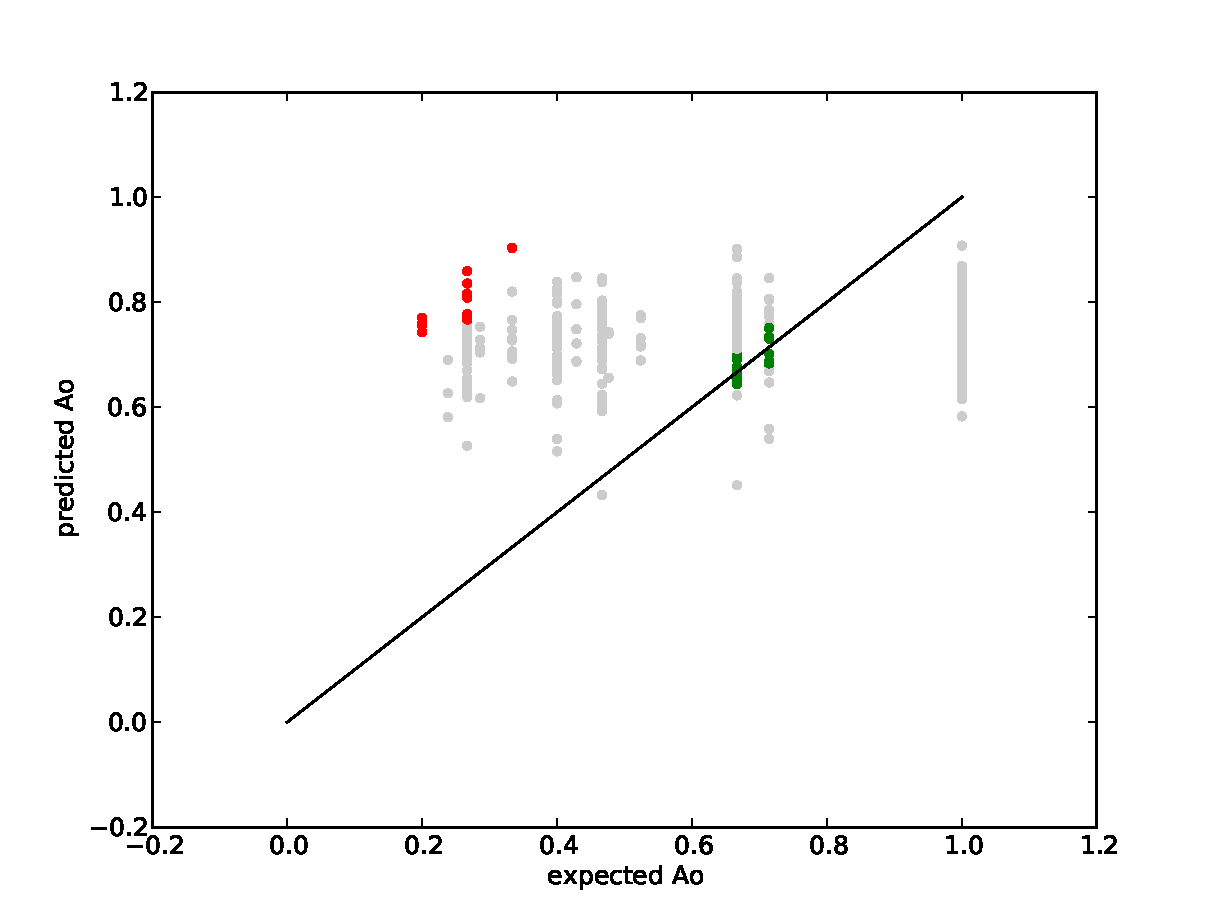
\includegraphics[scale=0.25]{scatterdraft.pdf}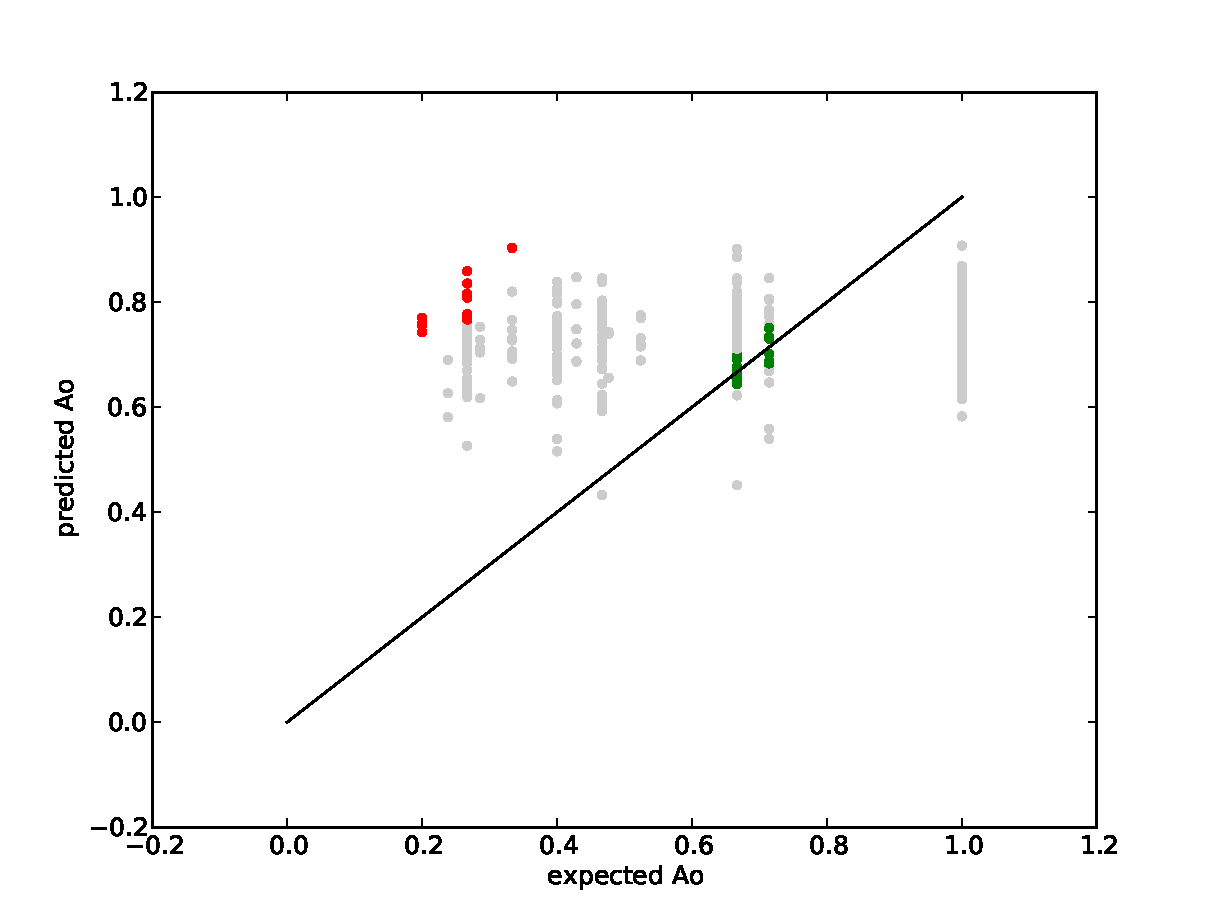
\includegraphics[scale=0.25]{scatterdraft.pdf}
%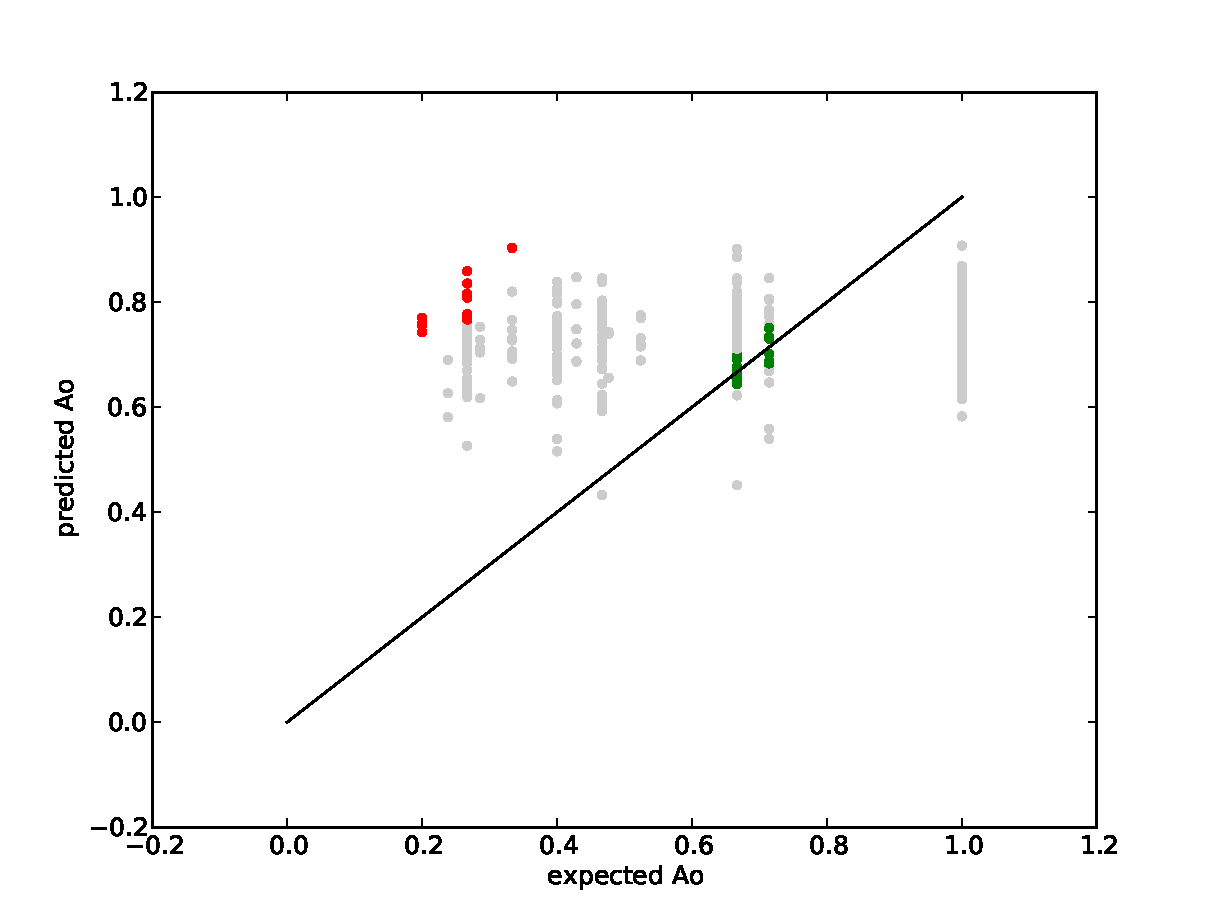
\includegraphics[scale=0.25]{scatterdraft.pdf}
%
%\caption{ \label{fig:reglit_dklocorg}\textcolor{red}{Comparative scatterplots for some datasets}}    
%\end{figure*}

% include your own bib file like this:
%\bibliographystyle{acl}
%\bibliography{acl2015}

\subsection{Feature analysis}


Figure \ref{fig:correlations} shows the Spearman correlation with $A_o$ for the numeric features on two English datasets, namely \textsc{mascc} and \textsc{fntw}. Even though there is variation in the magnitude across datasets, we observe strong negative correlation of the sense inventory features (\textit{z\_senseentropy}, \textit{z\_nlabels}), but also for the frequency of the target word (\textit{a\_targetfreq}). Notice that these features are also colinear, and in word-sense annotation high-frequency words can be partly more difficult to annotate because they can be more polysemous. 

Given these correlations, the feature repertoire we use captures better the low-agreement area of the data, but no feature has a consistently high posi\-tive correlation with agreement. That is, the predictors for low-agreement are more reliable than those for high agreement. 

A possible candidate for high-agreement prediction could be the proportion of content words over the length of the context, arguably because more lexically rich context are easier to desambiguate by the annotators. This feature has a positive value for most datasets except \textsc{mascc}. This property has already been noted by \newcite{passonneau2009making}, who mention that `greater specificity in the contexts of use leads to higher agreement'.
\begin{figure*}[htt]
\begin{center}
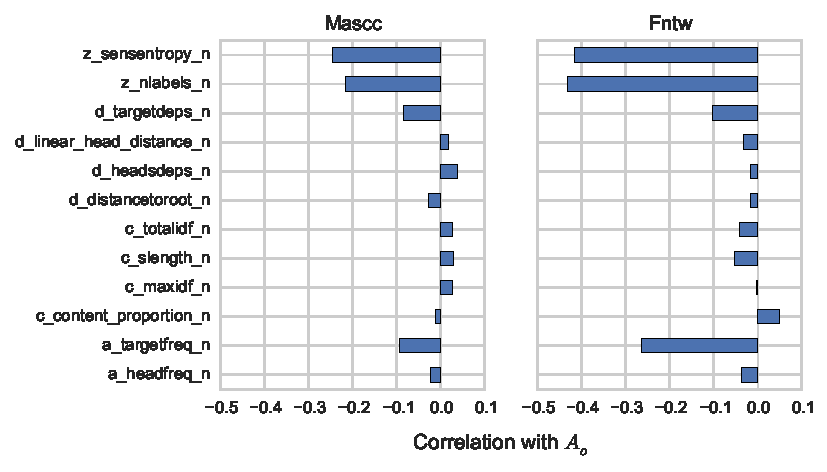
\includegraphics[scale=1.0]{mascc_fntw_a0_correlation.pdf}

\end{center}\caption{ \label{fig:correlations}Correlation between the numeric-valued features and $A_o$ for \textsc{mascc} and \textsc{fntw}}    
\end{figure*}

Syntactic complexity is also an indicator of difficulty. Words with many dependents  are often more difficult to annotate (\textit{d\_targetdeps} has a consistently negative correlation with $A_o$), while words with many syntactic siblings  are placed in more specific contexts and are easier to annotate, giving \textit{d\_headdeps} a slight positive correlation with $A_o$. This behavior holds for all the English datasets except \textsc{mascc}, as well as for \textsc{eusc}.

We have also performed group-wise feature ablation tests on regression and classification, with similar results. Based on the contribution of single feature groups, we find that the sense-inventory group constantly outperforms the other groups, followed by the morphology group. 
When the sense inventory is ignored from the features, performance almost always decreases, indicating that sense inventory information is very valuable to predict agreement. However, context information is necessary to distinguish between examples of the same word (say, in a one-lemma lexical-sample dataset), where the sense-inventory features would be constant across the whole dataset. 

Similarly, in the class-based experiments of \newcite{alonso2013annotation}, certain features like plural or number of dependents are strong predictors for low agreement when annotating between the \textit{container} and the \textit{content} senses of words like \textit{bowl} and \textit{glass}. However,
our datasets are either all-words or groupings of lexical-sample annotations for different words (e.g.\ \textsc{masc2} contains examples of \textit{fair-j}, \textit{know-v}, \textit{land-n}, etc.), which means that some of the class- or lemma-dependent features might be swamped by the superposition of features from the other words.  

Nevertheless, the systems do not always improve when adding context features, which suggests that there is room for improvement in capturing contextual information for sense-annotated instances.
\section{Conclusions and further work}
%This article provides, to the best of our knowledge, the first attempt to predict instance-wise agreement across multiple sense-annotated task that are different in language, sense inventory 
This article addresses the prediction of  instance-wise agreement for sense-annotated data. 
We have described a method to model agreement as a continuous value, and as a set of three discrete values. We use a feature scheme that tries to give account for the lexical, morphologic and syntactic properties of the examples. We have conducted experiments on nine datasets, which comprise three languages, all-words vs. lexical-sample word annotations, and crowdsourced vs. expert annotations. 

%This system can be used as an automatic review method for sense-annotation tasks, because it identifies a proportion of systematic disagreement (in particular the low end of it) that can be attributed to certain linguistic features, which can lead to reviews of annotation guidelines. 

The overall conclusiveness of the study requires expanding this research to more datasets and languages, as well as further exploring the difference in annotator bias between expert and crowdsourced annotations. Our feature repertoire can be expanded with characteristics of the sense inventory in terms of sense relatedness like autohyponymy, depth in the sense ontology, or qualitative properties of the senses such abstractness. Context features can also be expanded by adding information from word sense induction and distributional models.

Moreover, if we are to examine agreement variation in full-document (as opposed to sentence-by-sentence) annotation, we suggest that document-level frequency would help concretize the meaning of a certain word, following the principle of one sense per discourse \cite{Gale1992}.

%If the numeric prediction of agreement is desirable over the three-way scheme we use for classification, it is worth considering alternative measures to $A_o$ that are more robust against singularities of the data such as the damaging effect in the pairwise comparisons of having many annotators. A possible candidate measure is annotation entropy \cite{Yarowsky2002}.


If the numeric prediction of agreement is desirable over classification, a metric like annotation entropy \cite{Lopez2015} is worth considering as an alternative measure to $A_o$, since it an information-theoretical measure that also gives account for distribution skewness. %is more robust against singularities of the data such as the damaging effect in the pairwise comparisons of having many annotators.


\bibliographystyle{acl}
\bibliography{biblio}

\end{document}
